
\section{Quantifying Feral Anomalies}
\label{sec:evaluation}

While many of the validations we encountered were I-confluent,
not all were. In this section, we specifically investigate the effect
of concurrent execution on two of the most popular non-I-confluent
validations: uniqueness and foreign key validations.

\subsection{Uniqueness Constraints and Isolation}

To begin, we consider Rails's uniqueness validations: 12.7\% of the
built-in validation uses we encountered. In this section, we discuss
how Rails implements uniqueness and show that this is---at least
theoretically---unsafe.

When a Model field is declared with a \texttt{:validates\_uniqueness}
annotation, any instance of that model is compared against all other
corresponding records in the database to ensure that the field is
indeed unique. ActiveRecord accomplishes this by issuing a
``\texttt{SELECT}'' query in SQL and, if no such record is found,
Rails updates the instance state in the database
(Appendix~\ref{sec:appendix-uniqueness-behavior}).

While this user-level uniqueness validation runs within a transaction,
the exact isolation level of the transaction affects its
correctness. For correct execution, the \texttt{SELECT} query must
effectively attain a predicate lock on the validated column for the
duration of the transaction. This behavior \textit{is} supported under
serializable isolation. However, under Read Committed or Repeatable
Read isolation, no such mutual exclusion will be performed, leading to
potential inconsistency.\footnote{Using \texttt{SELECT FOR UPDATE}
  under these weaker models would be safe, but Rails does not
  implement its predicate-based lookups as such (i.e., it instead opts
  for a simple \texttt{SELECT} statement).}  Moreover, under Snapshot Isolation,
insertions to different records will similarly result in
inconsistency.\footnote{The first reference to the potential integrity
  violations resulting from this implementation in the Rails code that
  we are aware of dates to December 2007, in Rails
  v.2.0.0~\cite{code-unique-race-one}.  In September 2008, another
  user added additional discussion within the code comments, noting
  that ``this could even happen if you use transactions with the
  'serializable' isolation
  level''~\cite{code-unique-race-two}. Without reading too closely,
  the use of ``'serializable''' possibly suggests familiarity with the
  common, erroneous labeling of Snapshot Isolation as ``serializable''
  (as in Oracle 12c documentation and PostgreSQL documentation prior
  to the introduction of SSI in version 9.1.1 in September
  2011)\label{fn:si-rails}. } Thus, unless the database is configured
for serializable isolation, inconsistency may result and the feral
validation will fail.

As we have discussed, MySQL and PostgreSQL each support serializable
isolation but default to weaker isolation. Moreover, in our
investigation, we discovered a bug in PostgreSQL's implementation of
Serializable Snapshot Isolation that allowed duplicate records to be
created under serializable isolation when running a set of
transactions derived from the Rails primary key validator. As of
February 2015 (PostgreSQL 9.3.5) have confirmed this behavior with the
core PostgreSQL developers.\footnote{``BUG \#11732: Non-serializable
  outcomes under serializable isolation'' at \url{http://www.postgresql.org/message-id/20141021071458.2678.9080@wrigleys.postgresql.org}\label{fn:pg-bug}} Thus, any discussion of weak isolation
levels aside, PostgreSQL's implementation of serializability is not
actually sufficient to provide correct behavior for the above
uniqueness validations. We note that so-called ``serializable''
databases such as Oracle 12c that actually provide Snapshot Isolation
will similarly fall prey to duplicate validations.

Interestingly, the Rails documentation actually warns that duplicate
records may be inserted even despite uniqueness
validations~\cite{rails-guide}. However, despite the existence of
patches that remedy this behavior by the use of an in-database
constraint and/or index, Rails provides this incorrect behavior out of
the box. (The patch was rejected; a developer reports ``[t]he reasons
for it not being incorporated...are lost in the mists of time but I
suspect it's to do with backwards compatibility, cross database
compatibility and applications varying on how they want/need to handle
these kind of errors.''~\cite{code-index-patch}).

In another bug report complaining of duplicates due to concurrent
uniqueness validation, a commenter asserts ``this is not a bug but
documented and inherent behavior of
validates\_uniqueness\_of''~\cite{code-index-error}.  A Rails
committer follows up, noting that ``the only way to handle
[uniqueness] properly is at the database layer with a unique
constraint on the column,'' and subsequently closes the issue. The
original bug reporter protests that ``the problem extends beyond
unique constraints and into validations that are unique to a Rails
application that can't [sic?!]  be enforced on the DB level''; the
Rails committer responds that ``with the possible exception of
[associations,] all of the other validations are constrained by the
attribute values currently in memory, so aren't susceptible to similar
flaws.'' This is an interesting claim, which we investigate in the
remainder of this section and further discuss in
Section~\ref{sec:discussion}.

\minihead{Understanding validation behavior} Given that entirely feral
mechanisms can introduce duplicates, how many duplicates can be
introduced? Once a record is written, any later validations will
observe it via \texttt{SELECT} calls. However, \textit{while} a record
is being validated, any number of concurrent validations can
(un)safely proceed. In practice, the number of concurrent validations
is dependent on the Rails environment. In a Rails deployment
permitting $P$ concurrent validations (e.g., a single-threaded,
multi-process environment with $P$ processes), each value in the
domain of the model field/database column can be inserted no more than
$P$ times. Thus, validations---at least theoretically---bound the
worst-case number of duplicate records for each unique value in the
database table.

\subsection{Quantifying Uniqueness Anomalies}

Given that feral uniqueness validations are $i.)$ acknowledged to be
broken (at least under non-serializable isolation), $ii.)$ have a
work-around by correctly declaring them within the database, yet
$iii.)$ are widely used, we sought to understand exactly how often
uniqueness anomalies occur in an actual deployment. In this section,
we show that uniqueness validations in Rails are indeed unsafe under
non-serializable isolation. While they prevent some data integrity
errors, we observe---depending on the workload---many duplicate
records to be created.

\minihead{Experimental setup} We developed a Rails 4.1.5 application
that performed insertions to a non-indexed string column and compared
the incidence of violations both with and without a uniqueness
validator (for more details, see
Appendix~\ref{sec:appendix-uniqueness-schema}).\footnote{In our
  experimental evaluation, we use the custom applications described
  below (and in Appendix~\ref{sec:appendix-experiments}) for two
  reasons. First, these test cases allow us to isolate ActiveRecord
  behavior to the relevant set of validations as they are deployed by
  default and independent of any specialized controller logic. Second,
  this reduces the complexity of programmatic deployment and testing;
  we are able to bypass sessionization and authentication logic when
  triggering ActiveRecord. Many of the applications in our corpus
  indeed use the same code paths within ActiveRecord, but, to, say,
  create a new user in an application (without modifying the actual
  application code) would otherwise require additional inputs,
  including a session and authorization token as well as email and/or
  Captcha authentication. These applications indeed allow concurrent
  accesses, but the process of actually producing concurrency using
  their native HTTP interfaces is more complex.} We deployed this
application across two Amazon EC2 \texttt{m2.4xlarge} instances,
offering 68.4 GB RAM, 8 CPU cores, and 1680GB local storage, running
Ubuntu 14.04 LTS. On one instance, we deployed our application, using
Nginx 1.6.2 as a web frontend proxied to a set of Unicorn 4.8.3 (Ruby
VM pool) workers. That is, Nginx acts as a HTTP frontend and forwards
incoming requests to a variably sized pool of Rails VMs (managed by
Unicorn, in a multi-process single-threaded concurrency model) that,
in effect, \texttt{epoll} on a shared Linux file descriptor. On the
other EC2 instance, we deployed PostgreSQL 9.3.5 and configured it to
run on the instance local storage. We used a third EC2 instance to
direct traffic to the front-end instance and drive load. We plot the
average and standard deviation of three runs per experiment.

\minihead{Stress test} We began our study by issuing a simple stress
test that executed a number of concurrent insertion requests against a
variable number of Unicorn workers. We repeatedly issued a set of 64
concurrent model creation (SQL insertion) requests, each with the same
validated key (e.g., all with field \texttt{key} set to value 1)
against the Rails application. Across an increasing number of Unicorn
workers, we repeated this set of requests 100 times (blocking
in-between rounds to ensure that each round is, in fact, a concurrent
set of requests), changing the validated key each round
(Appendix~\ref{sec:appendix-uniqueness-stress}).

Figure~\ref{fig:pk-stress} shows the results. With no validation, all
concurrent requests succeed, resulting in 6300 duplicate records (100
rounds of 64-1 duplicate keys). With validations enabled, the number
of violations depends on the degree of concurrency allowed by
Unicorn. With only one process, Unicorn performs the validations
serially, resulting in no duplicates. However, with two processes,
Unicorn processes begin to race, resulting in 70 duplicate records
spread across 70 keys. With three processes, Unicorn produces 249
duplicate records across all 100 keys. The number of duplicates
increases with the number of processes, maximizing at 16 worker
processes. With additional processes, duplicates slightly decrease,
which we attribute to thrashing between processes and within
PostgreSQL (given that each instance has only 8 cores). Nevertheless,
using validations, the microbenchmark duplicate count remains below
700---nearly an order-of-magnitude fewer duplicates than without using
validations. Therefore, even though these validations are, in fact,
incorrectly implemented, they still result in fewer
anomalies. However, when we added in in-database unique index on the
\texttt{key} column\footnote{In this case, we added a unique index to
  the model using Active Record's \textit{database migration}, or
  manual schema change functionality. Migrations are written
  separately from the Active Record model declarations. Adding the
  index was not difficult, but, nevertheless, the index addition logic
  is separate from the domain model. Without using third-party models,
  we are unaware of a way to enforce uniqueness within Rails without
  first declaring an index that is \textit{also} annotated with a
  special \texttt{unique: true} attribute.} and repeated the
experiment, we observed no duplicates, as expected.

\begin{figure}\vspace{-1em}
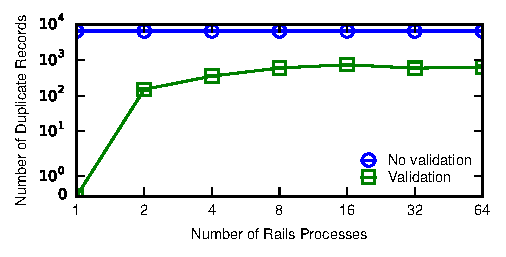
\includegraphics[width=\columnwidth]{figs/pk_stress_violations.pdf}\vspace{-1.5em}
\caption{Uniqueness stress test integrity violations.}
\label{fig:pk-stress}
\end{figure} 

\minihead{Actual workloads} The preceding experiment stressed a
particularly high-contention workload---in effect, a worst case
workload for uniqueness validations. In practice, such a workload is
likely rare.\footnote{In fact, it was in the above workload that we
  encountered the non-serializable PostgreSQL behavior under
  serializable isolation. Under serializable isolation, the number of
  anomalies is reduced compared to the number under Read Committed
  isolation (as we report here), but we still detected duplicate
  records.} Accordingly, we set up another workload meant to capture a
less pathological access pattern. We ran another insert-only workload,
with key choice distributed among a fixed set of keys. By varying the
distribution and number of keys, we were able to both capture more
realistic workloads and also control the amount of contention in the
workload. As a basis for comparison, we ran four different
distributions. First, we considered uniform key access. Second, we
used YCSB's Zipfian-distributed accesses from
\texttt{workloada}~\cite{ycsb}. Third and fourth, we used the item
distribution access from Facebook's LinkBench workload, which captures
MySQL record access when serving Facebook's social
graph~\cite{linkbench}. Specifically, we used---separately---the
insert and update traffic from this benchmark.

For each trial in this workload, we used 64 concurrent clients
independently issuing a set of 100 requests each, with a fixed number
of 64 Unicorn workers per process (Appendix~\ref{sec:appendix-uniqueness-workload}). 

Figure~\ref{fig:pk-workload} illustrates the number of duplicate
records observed under each of these workloads. As we increase the
number of possible keys, there are two opposing effects. With more
keys, the probability of any two operations colliding
decreases. However, recall that, once a key is written, all subsequent
validators can read it. While
the uniform workload observes an average of 2.33 duplicate records
with only one possible key, it observes an average of 26 duplicate
keys with 1000 possible keys. Nevertheless, with 1 million possible
keys, we do not observe any duplicate records.

The actual ``production'' workloads exhibit different trends. In
general, YCSB is an extremely high contention workload, with a Zipfian
constant of 0.99, resulting in one very hot key. This decreases the
beneficial effect of increasing the number of keys in the
database. However, LinkBench has less contention and anomalies decrease more
rapidly with increased numbers of keys.

\begin{figure}

\begin{minipage}[l]{0cm}

\includegraphics[angle=90, width=.185in]{figs/pk-workload-ylabel.pdf}
\end{minipage}
\begin{minipage}{\columnwidth}
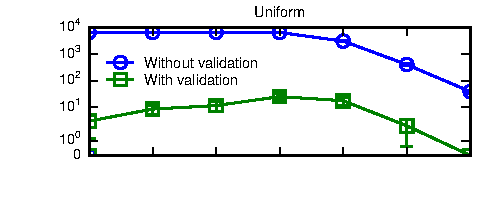
\includegraphics[width=1\columnwidth]{figs/pk-workload-uniform-violations.pdf}\vspace{-2em}
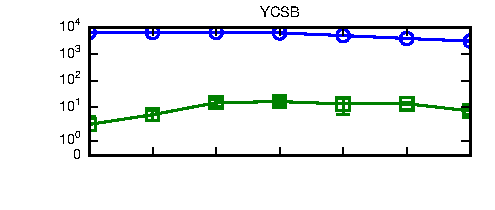
\includegraphics[width=1\columnwidth]{figs/pk-workload-ycsb-violations.pdf}\vspace{-2em}
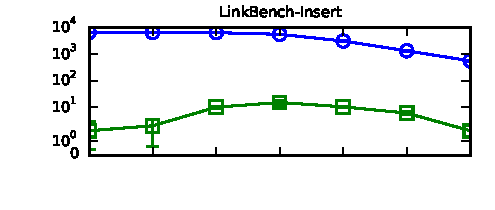
\includegraphics[width=1\columnwidth]{figs/pk-workload-linkbench-ins-violations.pdf}\vspace{-2em}
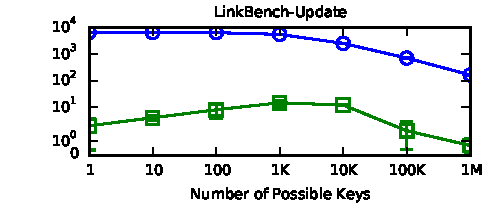
\includegraphics[width=1\columnwidth]{figs/pk-workload-linkbench-upd-violations.pdf}\vspace{-1em}
\end{minipage}
\caption{Uniqueness workload integrity violations.}
\label{fig:pk-workload}
\end{figure}

\subsection{Association Validations and Isolation}

Having investigated uniqueness constraints, we turn our attention to
association validations. We first, again, discuss how Rails enforces
these validations and describe how---at least
theoretically---validations might result in integrity errors.

When a Model field is declared with an association (e.g., it
\texttt{:belongs\_to} another model) \textit{and} a
\texttt{:validates\_presence} validation, Rails will attempt to ensure
that the declared validation is valid before saving the model. Rails
accomplishes this by issuing a ``\texttt{SELECT WHERE}'' query in SQL
to find an associated record (e.g., to ensure the ``one'' end of a
one-to-many relationship exists) and, if a matching association is
found, Rails updates the instance state in the database
(Appendix~\ref{sec:appendix-association-behavior}). On deletion, any
models with associations marked with \texttt{:dependent => destroy}
(or \texttt{:dependent => delete}) will have any associated models
destroyed (i.e., removed by instantiating in Rails and calling
\texttt{destroy} on the model) or deleted (i.e., removed by simply
calling the database's \texttt{DELETE} method).

This feral association validation runs within a transaction, but,
again the exact isolation level of the transaction affects its
correctness. For correct execution, the \texttt{SELECT} query must
also attain a predicate lock on the specific value of the validated
column for the duration of the transaction. Similar to the uniqueness
validator, concurrent deletions and insertions are unsafe under Read
Committed, Repeatable Read, and Snapshot Isolation. Thus, unless the
database is configured for serializable isolation, inconsistency may
result and the feral validation will fail to prevent data corruption.

Unlike uniqueness validations, there is no discussion of associations
and concurrency anomalies in the Rails documentation. Moreover, in
Rails 4.1, there is no way to natively declare a foreign key
constraint\footnote{Rails 4.2 added support for foreign keys via
  migration annotation (separate from Models; similarly to adding a
  unique index) in December 2014.}; it must be done via a third-party
library such as \texttt{foreigner}~\cite{foreigner} or
\texttt{schema\_plus}~\cite{schemaplus}. Only two applications
(\texttt{canvaslms} and \texttt{diaspora}) used \texttt{foreigner},
and only one application (\texttt{juvia}) used
\texttt{schema\_plus}. One application (\texttt{jobsworth}) used a
custom schema annotation and constraint generator.

\minihead{Understanding association behavior} Given that entirely
feral mechanisms can introduce broken associations, how many dangling
records can be introduced? Once a record is deleted, any later
validations will observe it via \texttt{SELECT} calls. However, in the
worst case, the feral cascading deletion on the one side of a
one-to-many relation can stall indefinitely, allowing an unlimited
number of concurrent insertions to the many side of the
relation. Thus, validations---at least theoretically---only reduce the
worst-case number of dangling records that were inserted prior to
deletion; any number of concurrent insertions may occur during
validation, leading to unbounded numbers of dangling records.

\subsection{Quantifying Association Anomalies}

Given this potential for errors, we again set out to quantify
integrity errors. We demonstrate that weak isolation can indeed lead
to data integrity errors in Rails' implementation of associations.

We performed another set of experiments to test association validation
behavior under concurrent insertions and deletions. Using the same
Unicorn and PostgreSQL deployment as above, we configured another
application to test whether or not Rails validations would correctly
enforce association-based integrity constraints. We consider an
application with two models: Users and Departments. We configure a
one-to-many relationship: each user \texttt{belongs\_to} a department,
and each department \texttt{has\_many} user
(Appendix~\ref{sec:appendix-association-schema}).

As a basic stress test, we initialize the database by creating 100
departments with no users. Subsequently, for each department in the
database, we issue a single request to delete the department along
with 64 concurrent requests to insert users in that department. To
correctly preserve the one-to-many relationship, the database should
either reject the deletion operation or perform a cascading deletion
of the department and any users (while rejecting any future user
creation requests for that department). We can quantify the degree of
inconsistency by counting the number of users left in the database who
have no corresponding department (Appendix~\ref{sec:appendix-association-stress}).

With associations declared in Rails, the Rails process performing the
deletion will attempt a cascading delete of users upon department
deletion. However, this cascade is performed, again, ferally---at the
application level. Thus, under non-serializable isolation, any user creation
events that are processed while the search for Users to delete is
underway will result in Users without departments.

Figure~\ref{fig:fk-stress} shows the number of ``orphaned'' Users
(i.e., Users without a matching Department) as a function of Rails
worker processes. With no constraints declared to Rails or to the
database, all User creations succeed, resulting in 6400 dangling
Users. With constraints declared in Rails (via a mix of validation and
association), the degree of inconsistency depends on the degree of
parallelism. Under the worst case, with 64 concurrent processes, the
validations are almost worthless in preventing integrity errors. In
contrast, when we declare a foreign key constraint within the
database\footnote{In this case, we introduced the constraint via SQL
  using a direct connection to the database. This change was
  straightforward but---like the unique index addition---was not
  reflected in the base Active Record models.}  and run the workload
again, we observe no inconsistency.

\begin{figure}
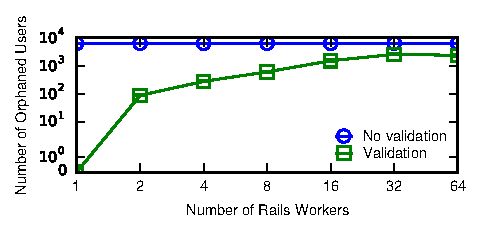
\includegraphics[width=\columnwidth]{figs/fk-stress-violations.pdf}\vspace{-1em}
\caption{Foreign key stress association anomalies.}
\label{fig:fk-stress}
\end{figure}

The above stress test shows that inconsistency due to feral
concurrency control occurs only during times of contention---parallel
deletions and insertions. We subsequently varied the degree of
contention within the workload. We configured the same application and
performed a set of insertions and deletions, but spread across a
greater number of keys and at random. A set of 64 processes
concurrently each issued 100 User creation and Department deletion
requests (at a ratio of 10 to 1) to a set of randomly-selected keys
(again at a ratio of 10 Users to each Department). By varying the
number of Users and Departments, we were able to control the amount of
contention within the workload. Under this workload, inconsistency
resulted only when a Department deletion proceeded concurrently with a
User creation event and the feral cascading deletion ``missed'' the
User creation (Appendix~\ref{sec:appendix-association-workload}).

Figure~\ref{fig:fk-workload} shows the results. As the number of
Departments increases, we observe two trends. First, with only one
Department, there is again less chance of inconsistency: all
operations contend on the same data item, so the total number of
inconsistent, orphaned users is limited by the number of potentially
racing. However, as the number of Departments increases, the chance of
concurrent deletions and insertions drops.

\begin{figure}
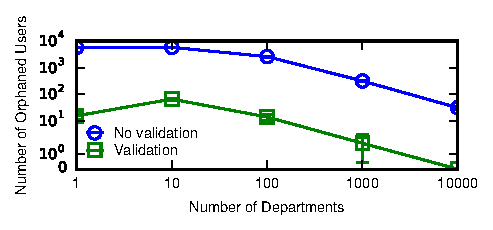
\includegraphics[width=\columnwidth]{figs/fk-workload-violations.pdf}\vspace{-1em}
\caption{Foreign key workload association anomalies.}
\label{fig:fk-workload}
\end{figure}

\subsection{Takeaways and Discussion}

The preceding experiments demonstrate that, indeed, Active Record is
unsafe as deployed by default. Validations are susceptible to data
corruption due to sensitivity to weak isolation anomalies. Moreover,
in PostgreSQL, current transaction support is insufficient to prevent
all anomalies.

This raises the question: why declare validations at all? As we
observe, validations protect against \textit{some} data
corruption. First, they correctly guard against
non-concurrency-related anomalies such as data entry or input
errors. For example, if a user attempts to reserve a username that was
previously chosen, a validation would succeed. The failures we observe
here are solely due to concurrent execution. Without concurrent
execution, validations are correct. Second, validations \textit{do}
reduce the incidence of inconsistency. Empirically, even under
worst-case workloads, these validations result in order-of-magnitude
reductions in inconsistency. Under less pathological workloads, they
may eliminate it. It is possible that, in fact, the
degree of concurrency and data contention within Rails-backed
applications simply does not lead to these concurrency races---that,
in some sense, validations are ``good enough'' for many applications.

Nevertheless, in both cases, Rails's feral mechanisms are a poor
substitute for their respective database counterparts---at least in
terms of integrity. We re-examine the Rails community's reluctance to
embrace these mechanisms in Section~\ref{sec:discussion}.

